\documentclass[10pt]{article}

\usepackage[margin=0.75in]{geometry}
\usepackage{amsmath,amsthm,amssymb,bm}
\usepackage{xcolor}
\usepackage{cancel}
\usepackage{graphicx}
\usepackage{changepage}
\usepackage{circuitikz}
\usepackage{pgfplots}
\usepackage{minted}
\usepackage{physics}
\usepackage{hyperref}
\usepackage{siunitx}
\usepackage{fontspec}
\usepackage{relsize}
\usepackage{subfig}
\usepackage{todonotes}
\usepackage{multicol, multirow, booktabs}
\usepackage[breakable]{tcolorbox}
\usepackage[inline]{enumitem}

\theoremstyle{definition}
\newtheorem{problem}{Problem}
\newtheorem{soln}{Solution}

\pgfplotsset{compat=newest}
\usetikzlibrary{lindenmayersystems}
\usetikzlibrary{arrows}
\usetikzlibrary{calc}
\usetikzlibrary{positioning, fit}
\usetikzlibrary{3d, perspective}

\definecolor{incolor}{HTML}{303F9F}
\definecolor{outcolor}{HTML}{D84315}
\definecolor{cellborder}{HTML}{CFCFCF}
\definecolor{cellbackground}{HTML}{F7F7F7}
\newcommand{\ui}{\hat{i}}
\newcommand{\uj}{\hat{j}}
\newcommand{\uk}{\hat{k}}
\newcommand{\ux}{\hat{\mathbf{x}}}
\newcommand{\uy}{\hat{\mathbf{y}}}
\newcommand{\uz}{\hat{\mathbf{z}}}
\newcommand{\uv}[1]{\hat{\bm{{#1}}}}
\newcommand{\pr}[1]{{#1^\prime}}
\newcommand{\pd}[2][]{{\frac{\partial^{#1}}{\partial {{#2}^{#1}}}}}
\newcommand{\dif}[2][]{{\frac{d^{#1}}{d{{#2}^{#1}}}}}
\pgfdeclarelayer{background}  
\pgfsetlayers{background,main}
\AtBeginDocument{\RenewCommandCopy\qty\SI}

\makeatletter
\newcommand{\boxspacing}{\kern\kvtcb@left@rule\kern\kvtcb@boxsep}
\makeatother
\newcommand{\prompt}[4]{
    \ttfamily\llap{{\color{#2}[#3]:\hspace{3pt}#4}}\vspace{-\baselineskip}
}

\newcommand{\thevenin}[2]{
  \begin{center}
    \begin{circuitikz} \draw
      (0,0) -- (2,0) to[battery1, l_=$V_{Th}\eq#1$] (2,2) 
      to[resistor, l_=$R_{Th}\eq#2$] (0,2)
      ;
      \draw [o-] (-.07,2.079);
      \draw [o-] (-.07,0.079);
    \end{circuitikz}
  \end{center}
}

\newcommand{\norton}[2]{
  \begin{center}
    \begin{circuitikz} \draw
      (0,0) -- (3,0) to[american current source, l_=$I_{N}\eq#1$] (3,2) -- (0,2) (2,0)
      to[resistor, l=$R_{N}\eq#2$] (2,2)
      ;
      \draw [o-] (-.07,2.079);
      \draw [o-] (-.07,0.079);
    \end{circuitikz}
  \end{center}
}

\DeclareMathOperator{\Div}{div}
\DeclareMathOperator{\Curl}{curl}
\DeclareMathOperator{\sgn}{sgn}

\newcommand{\highlight}[1]{\colorbox{yellow}{$\displaystyle #1$}}

\newcommand{\ti}[1]{\widetilde{#1}}

\newfontface{\Kaufmann}{Kaufmann}
\DeclareTextFontCommand{\kf}{\Kaufmann}
\newcommand{\scriptr}{\fontsize{12pt}{12pt}\kf{r}}

\newfontface{\KaufmannB}{Kaufmann Bd BT}
\DeclareTextFontCommand{\kfb}{\KaufmannB}
\newcommand{\bscriptr}{\fontsize{12pt}{12pt}\kfb{r}}
\newcommand{\justif}[2]{&{#1}&\text{#2}}
\newcommand{\bv}[1]{\mathbf{#1}}

\title{Physics 3200Y: Assignment IV}
\author{Jeremy Favro (0805980) \\ Trent University, Peterborough, ON, Canada}
\date{\today}

\begin{document}
\maketitle

% PROBLEM 1
\begin{problem}
Three point charges are located as shown, each a distance $a$ from the origin.
Find the approximate electric field at points far from the origin. Express your answer
in spherical coordinates, and include the two lowest orders in the multipole expansion.
\begin{center}
  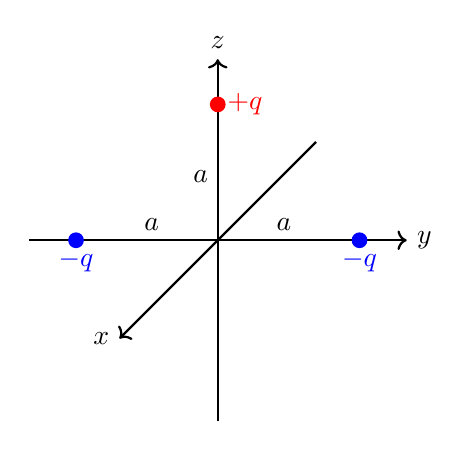
\begin{tikzpicture}[y={(0.5cm,0)},x={(-0.24cm,-0.24cm)},z={(0,0.5cm)}]
    \def\R{0.2}
    \def\L{4}
    \def\ymax{1.2*\L}
    \def\xmax{1.3*\L}
    \def\zmax{4.6}
    \coordinate (Q+) at (0,0,0.75*\zmax);
    \coordinate (Q-) at (0,0.75*\ymax,0);
    \coordinate (Qp-) at (0,-0.75*\ymax,0);

    % AXES
    \draw[->,thick] (-\xmax,0,0) -- (\xmax,0,0) node[left] {$x$};
    \draw[->,thick] (0,-\ymax,0) -- (0,\ymax,0) node[right] {$y$};
    \draw[->,thick] (0,0,-\zmax) -- (0,0,\zmax) node[above] {$z$};
    \node[above] at (0,0.35*\ymax,0) {$a$};
    \node[above] at (0,-0.35*\ymax,0) {$a$};
    \node[left] at (0,0,0.35*\zmax) {$a$};

    % CHARGE
    \fill[red,canvas is yz plane at x=0] (Q+) circle (\R) node[right] {$+q$};
    \fill[blue,canvas is yz plane at x=0] (Q-) circle (\R) node[below] {$-q$};
    \fill[blue,canvas is yz plane at x=0] (Qp-) circle (\R) node[below] {$-q$};
  \end{tikzpicture}
\end{center}
\end{problem}
\begin{soln}
  This configuration has net charge $-q$ so the monopole term will be nonzero. Explicitly for
  large distances from the charge configuration,
  $$\bv{E}_m\approx\frac{-q}{4\pi \epsilon_0r^2}\uv{r}.$$
  We then need the second order term for which we need to determine the dipole moment,
  \begin{align*}
    \bv{p} & =\sum_iq_i\pr{\bv{r}}_i                                        \\
           & =(-q)(-a)\uy+(-q)(a)\uy+(q)(a)\uz                              \\
           & =qa\uz=qa\left(\cos\theta\uv{r}+\sin\theta \uv{\theta}\right).
  \end{align*}
  Then in order to determine the electric field we need the dipole potential,
  $$V_d(\uv{r})=\frac{\bv{p}\cdot\bscriptr}{4\pi\epsilon_0\scriptr^2}\approx\frac{qa\left(\cos\theta\uv{r}+\sin\theta \uv{\theta}\right)\cdot \uv{r}}{4\pi\epsilon_0r^2}=\frac{qa\cos\theta}{4\pi\epsilon_0r^2}.$$
  Then the electric field is
  $$\bv{E}_d=-\bv{\nabla}V_d
    =-\frac{\partial}{\partial r}\frac{qa\cos\theta}{4\pi\epsilon_0r^2}\uv{r}-\frac{1}{r}\frac{\partial }{\partial \theta}\frac{qa\cos\theta}{4\pi\epsilon_0r^2}\uv{\theta}
    =-\frac{qa\cos\theta}{2\pi\epsilon_0r^3}\uv{r}+\frac{qa\sin\theta}{4\pi\epsilon_0r^3}\uv{\theta}.
  $$
  Now because electric fields obey linear superposition we can just find the total field as
  $$\bv{E}=\bv{E}_m+\bv{E}_d\approx \frac{-q}{4\pi \epsilon_0r^2}\uv{r}-\frac{qa\cos\theta}{2\pi\epsilon_0r^3}\uv{r}+\frac{qa\sin\theta}{4\pi\epsilon_0r^3}\uv{\theta}$$
\end{soln}
\newpage

% PROBLEM 2
\begin{problem}
The goal of this problem is to find the potential outside a long metal pipe of radius $a$. Put the axis of the pipe
along the $z$ axis, and let there be an external field $\bv{E}_0 = E_0\ux$. The total field is the sum of the external field
and the induced field due to the pipe. To solve this problem,
\begin{enumerate}[label=(\alph*)]
  \item List the boundary conditions.
  \item Solve Laplace's equation in cylindrical coordinates using separation of variables.
  \item Apply the boundary conditions to find the coefficients in your solution.
  \item Your final answer will look like
        $$V(s,\theta)=\sum_nA_nf_n(s,\phi)$$
        where $A_n$ are your coefficients and $f_n(s,\phi)$ are the orthogonal functions you obtained from Laplace's equation.
        \begin{enumerate}[label=\roman*.]
          \item Write a python function that takes as input $n$, $s$, and $\phi$ and returns the value of $f_n(s,\phi)$.
          \item Write a python code that uses this function to make a plot of the potential in the $xy$ plane for $s > a$.
        \end{enumerate}
\end{enumerate}
\end{problem}
\begin{soln}~
  \begin{enumerate}[label=(\alph*)]
    \item ~\begin{enumerate}[label=(\arabic*)]
            \item Since the pipe is a conductor it is also an equipotential. I'll say that the potential
                  at which the pipe sits is zero. Formally, $V(s=a,\theta)=0$.
            \item At large distances from the pipe the potential will be dominated by the external electric field.
                  Formally, $V(s\gg a,\theta)=-E_0x=-E_0s\cos\phi$.
            \item Since we want a physical (e.g. continuous) potential the potential must meet back up with itself
                  when we rotate about $z$.
          \end{enumerate}
    \item For a potential which does not depend on $\phi$ as we have here, Laplace's equation looks like
          $$\bv{\nabla}^2V=\frac{1}{s}\pd{s}\left(s\pd{s}V\right)+\frac{1}{s^2}\pd[2]{\phi}V=0.$$
          Using separation of variables we are looking for solutions of the form
          $$V(s,\phi)=S(s)\Phi(\phi)$$
          and so our Laplacian becomes
          $$\frac{1}{s}\pd{s}\left(s\pd{s}S(s)\Phi(\phi)\right)+\frac{1}{s^2}\pd[2]{\phi}S(s)\Phi(\phi)=0$$
          which we can rearrange to
          $$\frac{s}{S(s)}\dif{s}\left(s\dif{s}S(s)\right)+\frac{1}{\Phi(\phi)}\dif[2]{\phi}\Phi(\phi)=0.$$
          Now in order to actually separate the variables we must choose a side to be negative. We want
          solutions which are continuous in all variables and so must choose the $\phi$ term to be the negative one else we would
          obtain a differential equation which would yield (real valued) exponentials which do not circle back around to their original value when adding
          $2\pi$ to their argument. So we have now
          $$\frac{s}{S(s)}\dif{s}\left(s\dif{s}S(s)\right)=C;\qquad -\frac{1}{\Phi(\phi)}\dif[2]{\phi}\Phi(\phi)=C.$$
          Solving these two ODEs now,
          $$\dif[2]{\phi}\Phi(\phi)=-C\Phi(\phi)\implies \Phi(\phi)=A\cos(k\phi)+B\sin(k\phi),\quad C=k^2$$
          and
          \begin{align*}
            0 & =s\dif{s}\left(s\dif{s}S(s)\right)-k^2S(s)           \\
              & =s\left(\dif{s}S(s)+s\dif[2]{s}S(s)\right)-k^2S(s)   \\
              & =\left(s\dif{s}S(s)+s^2\dif[2]{s}S(s)\right)-k^2S(s) \\
              & =s^2\dif[2]{s}S(s)+s\dif{s}S(s)-k^2S(s)              \\
          \end{align*}
          which is a Cauchy-Euler equation and can be solved by letting $S(s)=s^n$ and solving the quadratic in $n$ that results,
          $$
            n^2+(1-1)n-k^2=0\implies
            n=\frac{0\pm\sqrt{0-4(1)(-k^2)}}{2}
            =\pm k
          $$
          (assuming $k\geq0$). So our solution is of the form
          $$S(s)=Ds^{k}+Es^{-k}.$$
          Now applying our boundary conditions we first note that our requirement
          that $\Phi(\phi)=\Phi(\phi+2\pi)$ means that
          \begin{align*}
            A\cos(k\phi)+B\sin(k\phi) & =A\cos(k\phi+2k\pi)+B\sin(k\phi+2k\pi)                                                             \\
                                      & =A(\cos(k\phi)\cos(2k\pi)-\sin(k\phi)\sin(2k\pi))+B(\sin(k\phi)\cos(2k\pi)+\cos(k\phi)\sin(2k\pi))
          \end{align*}
          which means that $k$ must be an integer so that the terms with a $2k\pi$ argument drop out.
          $k=0$ is also allowed as $\Phi(\phi)=A$ is a valid solution.
          $k=0$ also gives us an entirely new ODE for both $\Phi(\phi)$ and $S(s)$ aside from the constant solutions,
          $$\dif[2]{\phi}\Phi(\phi)=0\implies \Phi(\phi)=F\phi+G$$
          and
          $$s^2\dif[2]{s}S(s)+s\dif{s}S(s)=0$$
          which is still Cauchy-Euler it just now has a repeated root and so
          $$S(s)=H\ln(s)+I.$$
          Note that in our solution
          $$\Phi(\phi)=F\phi+G$$
          $F=0$ as otherwise the solution does not obey boundary condition (3).
          With this we have enough information to write the full solution in a general form,
          \begin{align*}
            V(s,\phi) & =A+B\ln(s)+\sum_{k=1}^{\infty}s^k(C\cos(k\phi)+D\sin(k\phi))+s^{-k}(E\cos(k\phi)+F\sin(k\phi))                      \\
                      & =A+B\ln(s)+\sum_{k=1}^{\infty}Cs^k\cos(k\phi)+Ds^k\sin(k\phi)+Es^{-k}\cos(k\phi)+Fs^{-k}\sin(k\phi)                 \\
                      & =A+B\ln(s)+\sum_{k=1}^{\infty}\left(Cs^k+\frac{E}{s^k}\right)\cos(k\phi)+\left(Ds^k+\frac{F}{s^k}\right)\sin(k\phi) \\
          \end{align*}
          where we've merged all the constant terms out front into one, $A$ and multiplied through by the constants in from of
          the $S(s)$ solution terms.
          Now we can apply our boundary conditions. Beginning with (2),
          \begin{align*}
            -E_0s\cos\phi & =\lim_{s\to\infty} A+B\ln(s)+\sum_{k=1}^{\infty}\left(Cs^k+\frac{E}{s^k}\right)\cos(k\phi)+\left(Ds^k+\frac{F}{s^k}\right)\sin(k\phi) \\
                          & =\lim_{s\to\infty} A+B\ln(s)+\sum_{k=1}^{\infty}\left(Cs^k\right)\cos(k\phi)+\left(Ds^k\right)\sin(k\phi)
          \end{align*}
          For this to not blow up we must have that $B=0$. Additionally, by inspection, to match the LHS and RHS the only $k$ value we can accept
          is $k=1$ so $D=C=0$ (and $A=0$) for $k\neq 1$ and in fact $D=0$ always as there is no $\sin\phi$ term on the LHS. By the same logic $C=-E_0$. Hence,
          $$V(s,\phi)=\left(-E_0s+\frac{E}{s}\right)\cos(\phi).$$
          Now applying boundary condition (1) we obtain that
          $$
            V(a,\phi)=\left(-E_0a+\frac{E}{a}\right)\cos(\phi)=0
            \implies E\cos(\phi)=E_0a^2\cos(\phi).
          $$
          We have our full solution now,
          $$V(s,\phi)=E_0\left(-s+\frac{a^2}{s}\right)\cos(\phi)$$
    \item Done in (b)
          \newpage
    \item Note that the colorbar is only included to show sign and relative magnitude.\\
          \includegraphics[scale=0.5]{q2.png}
          \inputminted[
            frame=lines,
            framesep=2mm,
            baselinestretch=1.2,
            fontsize=\footnotesize,
            linenos,
            breaklines
          ]{python3}{potential_plot.py}
  \end{enumerate}
\end{soln}
\newpage

% PROBLEM 3
\begin{problem}
A line of charge extends along the $z$-axis from $z = -a$ to $z = a$. The linear charge density is
$$\lambda(z)=\begin{cases}
    -\lambda_0 & z<0 \\
    \lambda_0  & z>0
  \end{cases}$$
\begin{enumerate}[label=(\alph*)]
  \item Find, by direct integration of Griffiths Eq. (2.30), the potential $V(z)$ for $|z| > a$. Note that you have to
        handle positive and negative values of $z$ separately.
  \item This problem has azimuthal symmetry, which means that the potential can also be represented by
        Eq. (3.65). Find the unknown coefficients by matching the potential to the one you found in part (a).
        Make sure your solution works for both $z > 0$ and $z < 0$.
  \item \textbf{Bonus}. Plot your potential in the $xz$ plane. You will find the \texttt{scipy.special.legendre} module to be
        useful.
\end{enumerate}
\end{problem}
\begin{soln}~
  \begin{enumerate}[label=(\alph*)]
    \item Griffiths Eq. (2.30) is
          $$V=\frac{1}{4\pi\epsilon_0}\int\frac{\lambda(\pr{\bv{r}})}{\scriptr}\,d\pr{l}.$$
          In our case this integral splits up over the interval $[-a,a]$ as
          $$V=\frac{\lambda_0}{4\pi\epsilon_0}\left[-\int_{-a}^{0}\frac{1}{\abs{z-\pr{z}}}\,d\pr{z}+\int_0^a\frac{1}{\abs{z-\pr{z}}}\,d\pr{z}\right]$$
          which for $z<-a$ (we are restricted to $|z| > a$, so we remove the infinite ``puck'' which runs from $-a$ to $a$) becomes
          \begin{align*}
            V & =\frac{\lambda_0}{4\pi\epsilon_0}\left[-\int_{-a}^{0}\frac{1}{\pr{z}-z}\,d\pr{z}+\int_0^a\frac{1}{\pr{z}-z}\,d\pr{z}\right] \\
              & =\frac{\lambda_0}{4\pi\epsilon_0}\left[-\ln(-z)+\ln(-a-z)+\ln(a-z)-\ln(-z)\right]                                           \\
              & =\frac{\lambda_0}{4\pi\epsilon_0}\left[-\ln(z^2)+\ln(z^2-a^2)\right]                                                        \\
              & =\frac{\lambda_0}{4\pi\epsilon_0}\ln(\frac{z^2-a^2}{z^2})
          \end{align*}
          and for $z>a$,
          \begin{align*}
            V & =\frac{\lambda_0}{4\pi\epsilon_0}\left[-\int_{-a}^{0}\frac{1}{z-\pr{z}}\,d\pr{z}+\int_0^a\frac{1}{z-\pr{z}}\,d\pr{z}\right] \\
              & =\frac{\lambda_0}{4\pi\epsilon_0}\left[\ln(z)-\ln(z+a)-\ln(z-a)+\ln(z)\right]                                               \\
              & =\frac{\lambda_0}{4\pi\epsilon_0}\left[\ln(z^2)-\ln(z^2-a^2)\right]                                                         \\
              & =\frac{\lambda_0}{4\pi\epsilon_0}\ln(\frac{z^2}{z^2-a^2}).
          \end{align*}
    \item Eq. (3.65) is
          $$V=\sum_{\ell=0}^\infty (A_\ell r^\ell+\frac{B_\ell}{r^{\ell+1}})P_\ell(\cos\theta).$$
          I'm not sure if it's appropriate to match these two without saying that $r=z$ which I'm also not sure is correct (we'd also have $\cos\theta=1\implies P_\ell(1)=1$).
          However it feels okay enough so we'll do that and see where it goes.
          We are trying to match up the expressions
          $$V=\sum_{\ell=0}^\infty  (A_\ell z^\ell+\frac{B_\ell}{z^{\ell+1}})$$
          and (let's start with $z<-a$)
          $$V=\frac{\lambda_0}{4\pi\epsilon_0}\ln(\frac{z^2-a^2}{z^2}).$$
          The best way I can figure to do this is to expand both as sums,
          the first directly and the second as a Taylor series. We actually need to match the
          term-by-term integration of the series for the original integrand because doing it for the
          result of the integral is a mess (or I didn't figure out the right way to do it).
          This is
          \begin{align*}
            V & =\frac{\lambda_0}{4\pi\epsilon_0}\left[-\int_{-a}^{0}\frac{1}{\pr{z}-z}\,d\pr{z}+\int_0^a\frac{1}{\pr{z}-z}\,d\pr{z}\right]                                                                                \\
              & =\frac{\lambda_0}{4\pi\epsilon_0}\left[\int_{-a}^{0}\sum_{n=0}^{\infty}\left(\frac{\pr{z}^{n}}{z^{n+1}}\right)\,d\pr{z}-\int_0^a\sum_{n=0}^{\infty}\left(\frac{\pr{z}^{n}}{z^{n+1}}\right)\,d\pr{z}\right] \\
              & =\frac{\lambda_0}{4\pi\epsilon_0}\left[\eval{\sum_{n=0}^{\infty}\frac{\pr{z}^{n+1}}{(n+1)z^{n+1}}}_{-a}^{0}-\eval{\sum_{n=0}^{\infty}\frac{\pr{z}^{n+1}}{(n+1)z^{n+1}}}_{0}^{a}\right]                     \\
              & =\frac{\lambda_0}{4\pi\epsilon_0}\left[-\sum_{n=0}^{\infty}\frac{(-a)^{n+1}}{(n+1)z^{n+1}}-\sum_{n=0}^{\infty}\frac{a^{n+1}}{(n+1)z^{n+1}}\right]                                                          \\
              & =-\frac{\lambda_0}{4\pi\epsilon_0}\sum_{n=0}^{\infty}\frac{(-a)^{n+1}+a^{n+1}}{(n+1)z^{n+1}}
          \end{align*}
          which is zero for even $n$ and
          $$V=-\frac{\lambda_0}{4\pi\epsilon_0}\sum_{n=1,3,5,\dots}^{\infty}\frac{2a^{n+1}}{(n+1)z^{n+1}}$$
          otherwise.
          We can now match to the spherical solution potential!
          It is evident that $A_\ell=0$ as we have no terms where $z$ is in the numerator. Then
          $$B_\ell=-\frac{\lambda_0}{4\pi\epsilon_0}\frac{2a^{\ell+1}}{\ell+1}$$
          from our expression. So our solution in spherical is
          $$V=-\frac{\lambda_0}{4\pi\epsilon_0}\sum_{\ell=1,3,5,\dots}^{\infty}\frac{2a^{\ell+1}}{(\ell+1)z^{\ell+1}}$$
          for $z<-a$. For $z>a$ the process is much the same, we just have to flip the sign of the Taylor series in the integrals,
          \begin{align*}
            V & =\frac{\lambda_0}{4\pi\epsilon_0}\left[-\int_{-a}^{0}\frac{1}{\pr{z}-z}\,d\pr{z}+\int_0^a\frac{1}{\pr{z}-z}\,d\pr{z}\right]                                                                                 \\
              & =\frac{\lambda_0}{4\pi\epsilon_0}\left[-\int_{-a}^{0}\sum_{n=0}^{\infty}\left(\frac{\pr{z}^{n}}{z^{n+1}}\right)\,d\pr{z}+\int_0^a\sum_{n=0}^{\infty}\left(\frac{\pr{z}^{n}}{z^{n+1}}\right)\,d\pr{z}\right] \\
              & =\frac{\lambda_0}{4\pi\epsilon_0}\left[-\eval{\sum_{n=0}^{\infty}\frac{\pr{z}^{n+1}}{(n+1)z^{n+1}}}_{-a}^{0}+\eval{\sum_{n=0}^{\infty}\frac{\pr{z}^{n+1}}{(n+1)z^{n+1}}}_{0}^{a}\right]                     \\
              & =\frac{\lambda_0}{4\pi\epsilon_0}\left[\sum_{n=0}^{\infty}\frac{(-a)^{n+1}}{(n+1)z^{n+1}}+\sum_{n=0}^{\infty}\frac{a^{n+1}}{(n+1)z^{n+1}}\right]                                                            \\
              & =\frac{\lambda_0}{4\pi\epsilon_0}\sum_{n=0}^{\infty}\frac{(-a)^{n+1}+a^{n+1}}{(n+1)z^{n+1}}
          \end{align*}
          which is again zero for even $n$ and so we write it as
          $$V=\frac{\lambda_0}{4\pi\epsilon_0}\sum_{n=1,3,5,\dots}^{\infty}\frac{2a^{n+1}}{(n+1)z^{n+1}}$$
          which gives
          $$B_\ell=\frac{\lambda_0}{4\pi\epsilon_0}\frac{2a^{\ell+1}}{\ell+1}$$
          and gives the full solution to be
          $$V=\frac{\lambda_0}{4\pi\epsilon_0}\sum_{\ell=1,3,5,\dots}^{\infty}\frac{2a^{\ell+1}}{(\ell+1)z^{\ell+1}}.$$
          Since the signs of these expressions correspond nicely to the signs of $z$ we can just tack on a $\sgn(z)=z/\abs{z}$ out
          front and obtain a single solution which works for both regions:
          $$V=\frac{z}{\abs{z}}\frac{\lambda_0}{4\pi\epsilon_0}\sum_{\ell=1,3,5,\dots}^{\infty}\frac{2a^{\ell+1}}{(\ell+1)z^{\ell+1}}.$$
          \newpage
    \item Note that the potential axis is just to show relative scale and sign. The constant out front
          in the real potential would have a significant effect on the magnitude.\\
          \includegraphics[scale=0.5]{q3.png}
          \inputminted[
            frame=lines,
            framesep=2mm,
            baselinestretch=1.2,
            fontsize=\footnotesize,
            linenos,
            breaklines
          ]{python3}{potential_plot2.py}
  \end{enumerate}
\end{soln}

% PROBLEM 4
\begin{problem}
A sphere of radius $R$ carries a polarization
$$\bv{P}(\bv{r})=k\bv{r},$$
where $k$ is a constant and $\bv{r}$ the vector from the center of the sphere.
\begin{enumerate}[label=(\alph*)]
  \item Calculate the bound charges $\sigma_b$ and $\rho_b$.
  \item Find the electric field inside and outside the sphere.
\end{enumerate}
\end{problem}
\begin{soln}
  \begin{enumerate}[label=(\alph*)]
    \item $$\sigma_b=\bv{P}\cdot \hat{n}=\bv{P}\cdot\hat{r}=kR$$
          $$\rho_b=-\div{\bv{P}}=-\frac{1}{r^2}\pd{r}(kr^3)=-3k.$$
    \item For the inside of the sphere, $r<R$, we only consider the volume charge
          as the surface charge will self-cancel everywhere.
          The electric field due to $\rho_b$ is then, by Gauss' law,
          $$\bv{E}=\frac{1}{4\pi\epsilon_0}\frac{-3k\cdot\frac{4}{3}\pi r^3}{r^2}\uv{r}=-\frac{kr}{\epsilon_0}.$$
          Outside the sphere the field is zero as, again, by Gauss' law, $Q_{enc}$ is zero as the sphere has no net
          charge.
  \end{enumerate}
\end{soln}
\end{document}